% NetSci 2027 one-page abstract (layout follows the official NetSci2027 Overleaf template)
% Third draft, 23 November 2026. Single author, first person.
% To submit: open the NetSci2027 Abstract Template in Overleaf, paste the title, author, text, references and caption,
% upload figure.pdf, compile, and download the PDF.
\documentclass[10pt]{article}
\usepackage[letterpaper,margin=20mm]{geometry}
\usepackage[T1]{fontenc}
\usepackage{graphicx}
\IfFileExists{lmodern.sty}{\usepackage{lmodern}}{\usepackage{helvet}}
\renewcommand{\familydefault}{\sfdefault}
\pagestyle{empty}
\setlength{\parskip}{0.4\baselineskip}
\setlength{\parindent}{0pt}

\begin{document}

\begin{center}
{\Large\bfseries Weighted PageRank and Official Rankings in Tennis and Other Sports}\\[8pt]
{\normalsize Chakib Madcur}\\[3pt]
{\small Department of Computer Science, Roosevelt University, Chicago, IL, USA}
\end{center}

Official sports rankings follow different rules: tournament points in tennis, an Elo-type rating in international football, and league tables in team sports. Using ideas from network science, I rank competitors with weighted PageRank [1] on the directed network of match results, where every loser points to the winner and each link is weighted by the number of wins. I compare these PageRank rankings with the official rankings over five decades of men's and women's professional tennis [2,3], and in international football, the Premier League, the NBA, the NHL and the NFL. The two rankings are well correlated, so I focus on their differences. I compare their predictability by using each ranking at the end of one season to predict the winners of the next season's matches, and I examine where the rankings disagree: how much one upset of the world number one is worth, and which players gain or lose places depending on where and in which tournaments they play. The aim is to understand what each ranking rule rewards.

\begin{figure}[h]
\centering
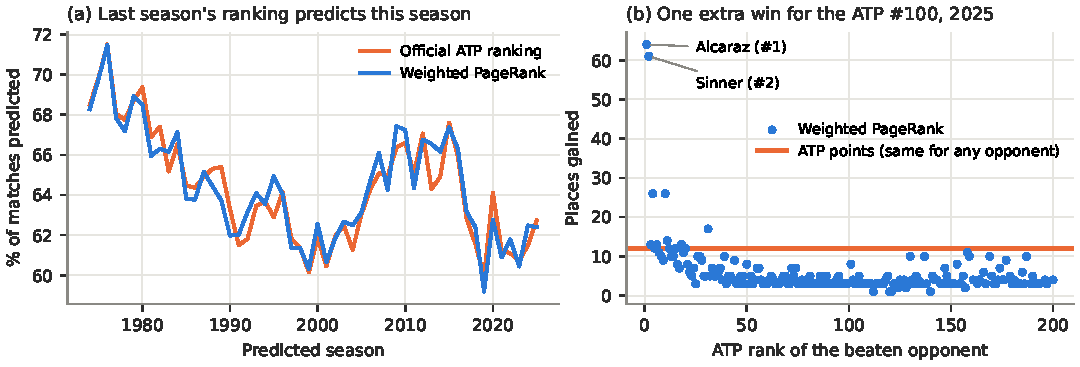
\includegraphics[width=\textwidth]{figure.pdf}
\caption{\small (a) Share of each season's ATP matches whose winner was ranked higher at the end of the previous season, by the official ATP ranking and by weighted PageRank. (b) Places gained in the 2025 rankings by the ATP number 100 from one extra win, by the ATP rank of the beaten opponent; the orange line is the gain under ATP points, which is the same for every opponent.}
\end{figure}

{\footnotesize
[1] S. Brin, L. Page, The anatomy of a large-scale hypertextual Web search engine, \emph{Computer Networks and ISDN Systems} 30, 107--117 (1998).\par
{}[2] F. Radicchi, Who is the best player ever? A complex network analysis of the history of professional tennis, \emph{PLoS ONE} 6, e17249 (2011).\par
{}[3] N. Dingle, W. Knottenbelt, D. Spanias, On the (Page) ranking of professional tennis players, in \emph{Computer Performance Engineering}, Springer (2013).\par}

\end{document}
